\documentclass[tikz, border=10pt]{standalone}
\usepackage{tikz}
\usetikzlibrary{positioning, calc}

\begin{document}

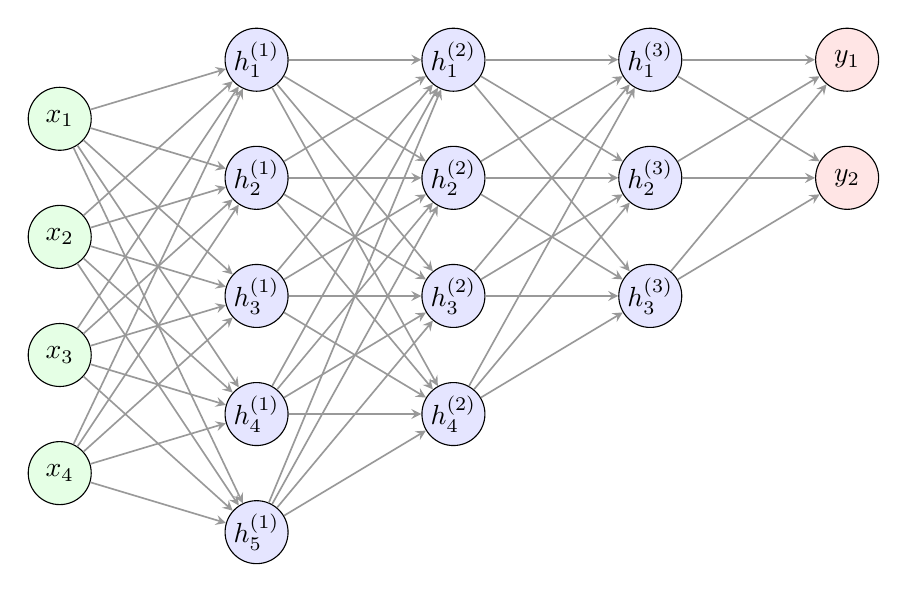
\begin{tikzpicture}[
    % 定义样式
    basic/.style={draw, fill=white, circle, minimum size=0.8cm, inner sep=0pt},
    input/.style={basic, fill=green!10},
    hidden/.style={basic, fill=blue!10},
    output/.style={basic, fill=red!10},
    arrow/.style={->, >=stealth, semithick, color=gray!80}
]

% --- 配置参数 ---
\def\inputnum{4}   % 输入层神经元数量
\def\hiddennumI{5} % 隐藏层1神经元数量
\def\hiddennumII{4}% 隐藏层2神经元数量
\def\hiddennumIII{3}% 隐藏层3神经元数量
\def\outputnum{2}  % 输出层神经元数量

% --- 绘制节点 ---

% 1. 输入层 (Input Layer)
\foreach \i in {1,...,\inputnum}
    \node[input] (I-\i) at (0, -\i*1.5) {$x_{\i}$};

% 2. 隐藏层 1 (Hidden Layer 1)
\foreach \h in {1,...,\hiddennumI}
    \node[hidden] (H1-\h) at (2.5, -\h*1.5 + 0.75) {$h^{(1)}_{\h}$};

% 3. 隐藏层 2 (Hidden Layer 2)
\foreach \h in {1,...,\hiddennumII}
    \node[hidden] (H2-\h) at (5, -\h*1.5 + 0.75) {$h^{(2)}_{\h}$};

% 4. 隐藏层 3 (Hidden Layer 3)
\foreach \h in {1,...,\hiddennumIII}
    \node[hidden] (H3-\h) at (7.5, -\h*1.5 + 0.75) {$h^{(3)}_{\h}$};

% 5. 输出层 (Output Layer)
\foreach \o in {1,...,\outputnum}
    \node[output] (O-\o) at (10, -\o*1.5 + 0.75) {$y_{\o}$};
% --- 绘制连接线 (Weights) ---

% 输入层 -> 隐藏层 1
\foreach \i in {1,...,\inputnum}
    \foreach \h in {1,...,\hiddennumI}
        \draw[arrow] (I-\i) -- (H1-\h);

% 隐藏层 1 -> 隐藏层 2
\foreach \h in {1,...,\hiddennumI}
    \foreach \k in {1,...,\hiddennumII}
        \draw[arrow] (H1-\h) -- (H2-\k);

% 隐藏层 2 -> 隐藏层 3
\foreach \h in {1,...,\hiddennumII}
    \foreach \k in {1,...,\hiddennumIII}
        \draw[arrow] (H2-\h) -- (H3-\k);

% 隐藏层 3 -> 输出层
\foreach \h in {1,...,\hiddennumIII}
    \foreach \o in {1,...,\outputnum}
        \draw[arrow] (H3-\h) -- (O-\o);

% % --- 添加层标签 ---
% \node[above=0.5cm of I-1, font=\bfseries] {Input Layer};
% \node[above=0.5cm of H1-1, font=\bfseries] {Hidden Layer 1};
% \node[above=0.5cm of H2-1, font=\bfseries] {Hidden Layer 2};
% \node[above=0.5cm of O-1, font=\bfseries] {Output Layer};

\end{tikzpicture}

\end{document}
